\documentclass[../../main.tex]{subfiles}
\begin{document}
\graphicspath{{figures/}{lectures/04_multinomial_lda/figures/}}
\section{Multinomial Logistic Regression \& LDA}
\begin{frame}[plain]
  \vfill\begin{center}{\Huge \textcolor{blue}{Multinomial Logistic Regression \& LDA}}\end{center}\vfill
\end{frame}
% Title Slide



%--------------------------------------------------
\begin{frame}{Multinomial Logistic Regression: Setup}
\small
We want to model
\[
p_k(x) = \Pr(Y=k \mid X=x), \quad k=1,\dots,K, \quad \sum_{k=1}^K p_k(x) = 1.
\]

\textbf{Idea:} Extend binary logistic regression ($K=2$) to multiple classes.  
We must ensure:
\begin{itemize}
    \item All probabilities $p_k(x)$ are nonnegative.
    \item They sum to 1 across all classes.
\end{itemize}

\textbf{Baseline coding:} Choose one class as reference (say class $K$).  
We model the log-odds of each class $k$ relative to the baseline:
\[
\log \frac{p_k(x)}{p_K(x)} = \beta_{k0} + \beta_{k1}x_1 + \cdots + \beta_{kp}x_p,
\quad k=1,\dots,K-1.
\]
\end{frame}

%--------------------------------------------------
\begin{frame}{Deriving the Probability Formula}
\small
From the log-odds definition:
\[
\frac{p_k(x)}{p_K(x)} = \exp(\beta_{k0} + \beta_{k1}x_1 + \cdots + \beta_{kp}x_p).
\]

Thus,
\[
p_k(x) = p_K(x) \cdot \exp(\beta_{k0} + \beta_{k1}x_1 + \cdots + \beta_{kp}x_p).
\]

Summing over all classes:
\[
1 = \sum_{j=1}^K p_j(x) 
= p_K(x) \Big( 1 + \sum_{l=1}^{K-1} \exp(\beta_{l0} + \beta_{l1}x_1 + \cdots + \beta_{lp}x_p) \Big).
\]

Therefore,
\[
p_K(x) = \frac{1}{1 + \sum_{l=1}^{K-1} e^{\beta_{l0} + \beta_{l1}x_1 + \cdots + \beta_{lp}x_p}}.
\]

And for $k=1,\dots,K-1$:
\[
p_k(x) = \frac{e^{\beta_{k0} + \beta_{k1}x_1 + \cdots + \beta_{kp}x_p}}{1 + \sum_{l=1}^{K-1} e^{\beta_{l0} + \beta_{l1}x_1 + \cdots + \beta_{lp}x_p}}.
\]
\end{frame}

%--------------------------------------------------
\begin{frame}{Interpretation of Coefficients}
\small
\textbf{Log-odds interpretation:}
\[
\log \frac{p_k(x)}{p_K(x)} = \beta_{k0} + \beta_{k1}x_1 + \cdots + \beta_{kp}x_p.
\]

\begin{itemize}
    \item $\beta_{kj}$ is the change in the \emph{log-odds} of being in class $k$ vs. baseline $K$ for a one-unit increase in $x_j$.
    \item Exponentiating:
    \[
    \frac{p_k(x)}{p_K(x)} \quad \text{changes by a factor of } e^{\beta_{kj}}
    \]
    for a one-unit increase in $x_j$.
\end{itemize}

\textbf{Example:}  
If baseline is \emph{epileptic seizure}, then:
\begin{itemize}
    \item $\beta_{\text{stroke},0}$ = log-odds of stroke vs. seizure when $x=0$.
    \item $\beta_{\text{stroke},j}$ = effect of $x_j$ on log-odds of stroke vs. seizure.
\end{itemize}
\end{frame}

%--------------------------------------------------
\begin{frame}{Softmax Formulation}
\small
An alternative (symmetric) parameterization avoids picking a baseline.  
This is widely used in ML (e.g., neural networks).

\textbf{Softmax probabilities:}
\[
p_k(x) = \frac{\exp(\beta_{k0} + \beta_{k1}x_1 + \cdots + \beta_{kp}x_p)}
{\sum_{l=1}^{K} \exp(\beta_{l0} + \beta_{l1}x_1 + \cdots + \beta_{lp}x_p)},
\quad k=1,\dots,K.
\]

\textbf{Log-odds ratio between class $k$ and $k'$:}
\[
\log \frac{p_k(x)}{p_{k'}(x)} =
(\beta_{k0} - \beta_{k'0}) + (\beta_{k1}-\beta_{k'1})x_1 + \cdots + (\beta_{kp}-\beta_{k'p})x_p.
\]

\begin{itemize}
    \item This shows that differences in coefficients determine relative odds between any two classes.
    \item Softmax ensures $\sum_k p_k(x)=1$ and $p_k(x)\geq 0$.
\end{itemize}
\end{frame}
%--------------------------------------------------

%--------------------------------------------------
\begin{frame}{Generative Models for Classification}
\begin{itemize}
    \item Logistic regression: models $\Pr(Y \mid X)$ directly (discriminative).  
    \item Generative approach: model $\Pr(X \mid Y)$ and $\Pr(Y)$, then use Bayes’ theorem:  
    \[
    \Pr(Y=k \mid X=x) = \frac{\pi_k f_k(x)}{\sum_{\ell=1}^K \pi_\ell f_\ell(x)}.
    \]
    \item Here:
    \begin{itemize}
        \item $\pi_k = \Pr(Y=k)$ = prior probability of class $k$.  
        \item $f_k(x) = \Pr(X=x \mid Y=k)$ = class-conditional density.  
    \end{itemize}
    \item Classify to the $k$ that maximizes $\Pr(Y=k \mid X=x)$ (Bayes classifier).  
\end{itemize}
\end{frame}

%--------------------------------------------------
\begin{frame}{Linear Discriminant Analysis: Assumptions}
\begin{itemize}
    \item Assume predictor distribution within each class is multivariate normal:
    \[
    X \mid Y=k \sim \mathcal{N}(\mu_k, \Sigma), \quad k=1,\dots,K.
    \]
    \item Common covariance matrix $\Sigma$ across all classes.  
    \item Then,
    \[
    f_k(x) = \frac{1}{(2\pi)^{p/2}|\Sigma|^{1/2}}
    \exp\!\left(-\tfrac{1}{2}(x-\mu_k)^T \Sigma^{-1}(x-\mu_k)\right).
    \]
    \item Plugging into Bayes’ rule yields a classifier with \textbf{linear decision boundaries}.
\end{itemize}
\end{frame}

%--------------------------------------------------
\begin{frame}{LDA Discriminant Functions}
\begin{itemize}
    \item Posterior log-probability (up to constant):
    \[
    \delta_k(x) = x^T \Sigma^{-1}\mu_k - \tfrac{1}{2}\mu_k^T \Sigma^{-1}\mu_k + \log \pi_k.
    \]
    \item LDA rule:
    \[
    \hat{Y} = \arg\max_k \delta_k(x).
    \]
    \item Properties:
    \begin{itemize}
        \item Boundaries between classes are hyperplanes (linear in $x$).  
        \item Incorporates both class means $\mu_k$ and priors $\pi_k$.  
        \item Effective when $p$ is moderate and normality assumption holds.  
    \end{itemize}
\end{itemize}
\end{frame}

%--------------------------------------------------
\begin{frame}{LDA Assumptions and Gaussian Density}
We want to classify an observation $X=x$ into one of $K$ classes.

\begin{block}{Key Assumption}
The class-conditional density is Gaussian:
\[
f_k(x) = \frac{1}{\sqrt{2\pi}\sigma_k} 
\exp\!\left( -\frac{1}{2\sigma_k^2}(x - \mu_k)^2 \right).
\]
\end{block}

\begin{itemize}
    \item $\mu_k$: class mean, $\sigma_k^2$: class variance.
    \item For simplicity, assume equal variance across classes:
    \[
    \sigma_1^2 = \cdots = \sigma_K^2 = \sigma^2.
    \]
\end{itemize}

This assumption leads to the \textbf{Linear Discriminant Analysis (LDA)} formulation.
\end{frame}

%--------------------------------------------------
\begin{frame}{Posterior Probabilities via Bayes' Rule}
From Bayes’ theorem, the posterior probability is
\[
p_k(x) = \Pr(Y=k \mid X=x) =
\frac{\pi_k f_k(x)}{\sum\limits_{l=1}^K \pi_l f_l(x)},
\]
where
\begin{itemize}
    \item $\pi_k = \Pr(Y=k)$ is the class prior,
    \item $f_k(x)$ is the class-conditional density.
\end{itemize}

Plugging in the Gaussian assumption:
\[
p_k(x) = 
\frac{\pi_k \,\frac{1}{\sqrt{2\pi}\sigma} 
\exp\!\left( -\frac{1}{2\sigma^2}(x - \mu_k)^2 \right)}
{\sum\limits_{l=1}^K \pi_l \,\frac{1}{\sqrt{2\pi}\sigma} 
\exp\!\left( -\frac{1}{2\sigma^2}(x - \mu_l)^2 \right)}.
\]
\end{frame}

%--------------------------------------------------
\begin{frame}{Linear Discriminant Functions}
We assign $x$ to the class with largest $p_k(x)$.  

Define the discriminant function by taking $\log$ of the numerator:
\[
\delta_k(x) = x \cdot \frac{\mu_k}{\sigma^2} 
- \frac{\mu_k^2}{2\sigma^2} + \log(\pi_k).
\]

\begin{itemize}
    \item Classification rule: assign $x$ to class with
    \[
    \delta_k(x) = \max_{j} \delta_j(x).
    \]
    \item The decision boundary between class $1$ and class $2$ occurs when
    \[
    \delta_1(x) = \delta_2(x).
    \]
\end{itemize}

\[
x = \frac{\mu_1 + \mu_2}{2}.
\]
\end{frame}

%--------------------------------------------------
\begin{frame}{Estimating Parameters for LDA}
In practice, the parameters are unknown.  

We estimate them from training data:

\[
\hat{\mu}_k = \frac{1}{n_k}\sum_{i:y_i=k} x_i,
\qquad
\hat{\sigma}^2 = \frac{1}{n-K}\sum_{k=1}^K \sum_{i:y_i=k}(x_i - \hat{\mu}_k)^2,
\]
\[
\hat{\pi}_k = \frac{n_k}{n}.
\]

\begin{block}{LDA Classifier}
Plugging in the estimates, the discriminant becomes
\[
\hat{\delta}_k(x) = x \cdot \frac{\hat{\mu}_k}{\hat{\sigma}^2} 
- \frac{\hat{\mu}_k^2}{2\hat{\sigma}^2} + \log(\hat{\pi}_k).
\]
Assign $x$ to the class with the largest $\hat{\delta}_k(x)$.
\end{block}
\end{frame}





\begin{frame}{Frame Title}
    \begin{figure}
    \centering
    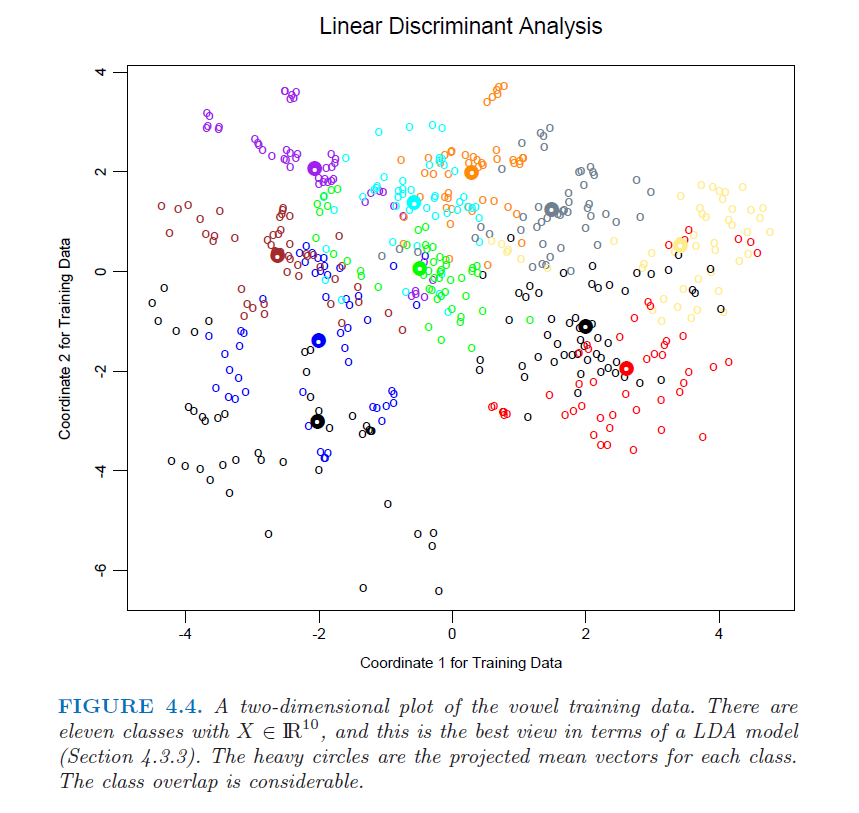
\includegraphics[width=0.5\linewidth]{lda_figure4_4.png}
    \caption{Elements of Statistical Learning, 2017}
    
\end{figure}
\end{frame}


\begin{frame}{Frame Title}

\begin{figure}
    \centering
    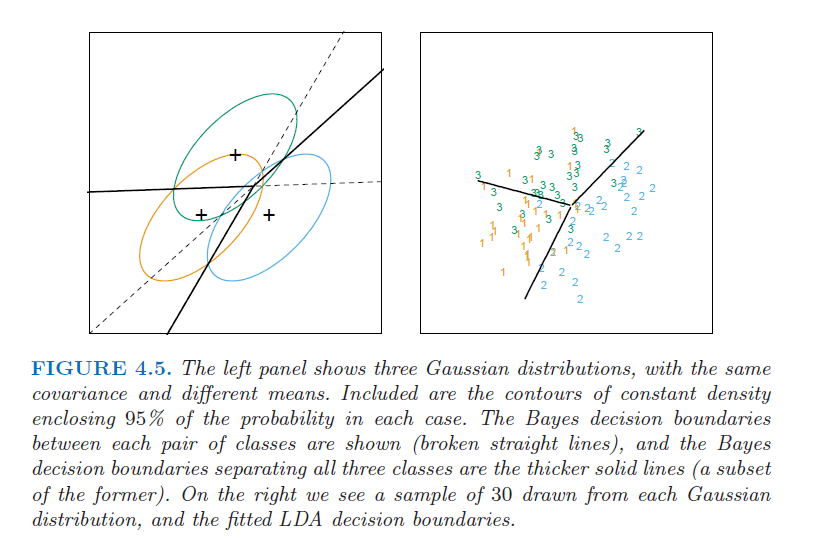
\includegraphics[width=0.5\linewidth]{figure4_5.png}
    \caption{Elements of Statistical Learning, 2017}
    
\end{figure}
\end{frame}
\end{document}
